% Template for Cogsci submission with R Markdown

% Stuff changed from original Markdown PLOS Template
\documentclass[10pt, letterpaper]{article}

\usepackage{cogsci}
\usepackage{pslatex}
\usepackage{float}
\usepackage{caption}

% amsmath package, useful for mathematical formulas
\usepackage{amsmath}

% amssymb package, useful for mathematical symbols
\usepackage{amssymb}

% hyperref package, useful for hyperlinks
\usepackage{hyperref}

% graphicx package, useful for including eps and pdf graphics
% include graphics with the command \includegraphics
\usepackage{graphicx}

% Sweave(-like)
\usepackage{fancyvrb}
\DefineVerbatimEnvironment{Sinput}{Verbatim}{fontshape=sl}
\DefineVerbatimEnvironment{Soutput}{Verbatim}{}
\DefineVerbatimEnvironment{Scode}{Verbatim}{fontshape=sl}
\newenvironment{Schunk}{}{}
\DefineVerbatimEnvironment{Code}{Verbatim}{}
\DefineVerbatimEnvironment{CodeInput}{Verbatim}{fontshape=sl}
\DefineVerbatimEnvironment{CodeOutput}{Verbatim}{}
\newenvironment{CodeChunk}{}{}

% cite package, to clean up citations in the main text. Do not remove.
\usepackage{cite}

\usepackage{color}

% Use doublespacing - comment out for single spacing
%\usepackage{setspace}
%\doublespacing


% % Text layout
% \topmargin 0.0cm
% \oddsidemargin 0.5cm
% \evensidemargin 0.5cm
% \textwidth 16cm
% \textheight 21cm

\title{Did I really do well? Young children are sensitive to the
informativeness of others' praise and use it to evaluate their own work}


\author{{\large \bf Mika Asaba},  {\large \bf Emily Hembacher}, {\large \bf Helen Qiu}, {\large \bf Brett Anderson}, {\large \bf Michael Frank}, {\large \bf Hyowon Gweon} \\ Department of Psychology, Stanford University}

\begin{document}

\maketitle

\begin{abstract}
Young children constantly receive praise about their abilities, skills,
and products. While much work has been devoted to how praise influences
children's motivation and self-esteem, an open question is how children
evaluate praise from others and use it to assess their own work. Given
young children's ability to track informant's accuracy and selectively
trust those who are more reliable, we examine their ability to monitor
the informativeness of others' praise. In particular, this work
investigates whether young children weight evaluations from a teacher
who provides praise with respect to the quality of a piece of work
higher than evaluations from a teacher who always provide praise. We
show that a dults (Experiment 1) and even 4-5 year-olds (Experiment 2)
show sensitivity to the difference in informativeness between these two
teachers, even when controlling for the frequency of praise (Experiment
3). These findings provide evidence that from a young age, children can
selectively use others' praise to evaluate their own work.

\textbf{Keywords:}
praise, theory of mind, uncertainty
\end{abstract}

One of the challenges of early childhood is learning about one's
abilities, traits, skills, and weaknesses, and an important source of
information is others' evaluations. Performance praise -- positive
evaluations of a person's performances or attributes (see Kanouse,
Gumpert, \& Canavan-Gumpert, 1981) -- has become ubiquitous in parenting
and education practices in Western societies. In order to make
appropriate inferences about their abilities and products, children must
learn to figure out when praise is meaningful and when it should be
discounted. Here, we examine children's sensitivity to the
\textit{informativeness} of praise and if so, whether children are
strategic in how they use praise to assess their own work.

However, while much work has been devoted to how praise influences
children's self-esteem (e.g., Brummelman, Thomaes, Orobio de Castro,
Overbeek, \& Bushman, 2014), intrinsic motivation (see Henderlong \&
Lepper, 2002 for a review), and learning behaviors (e.g., Mueller \&
Dweck, 1998), one open question is how young children might evaluate the
\textit{informational value} of praise depending on who it comes from.
As adults, we intuitively understand that not all praise carries equal
weight: people may vary in their competence, expertise, or communicative
goals (Yoon, Tessler, Goodman, \& Frank, 2016) and we should take these
factors into consideration when interpreting praise.

For instance, imagine that you are trying out different cookie recipes
and you ask two of your friends, Anne and Sally, what they think. You
remember that Anne usually tries to be nice and says that everything
tastes good, but Sally tends to provide more helpful, honest feedback
and only says that something tastes good if she really believes it
tastes good. Given this, you might interpret each friend's praise
differently: if Anne says she likes the cookies, then you might not
learn that much about the quality of the cookie itself, but if Sally
says she likes it, then you might infer that the cookie is really good.
In the current work, we examine whether young children share these
intuitions, in particular whether they can (1) track the informativeness
of others' praise from prior observations and (2) how they use might
others' informativeness to appropriately evaluate their own work.

Some prior work has argued that children may perceive praise as
insincere when it is overly general or inconsistent with how the child
views herself, especially when the child can think of counterexamples to
the evaluation (see Henderlong \& Lepper, 2002). While the consistency
between the child's and informant's evaluation of a product the child
created could provide cues to sincerity, children can also observe
whether the contingency of an informant's praise on quality to determine
who to trust for evaluative information.

In fact, young children are quite savvy in judging the information that
others provide, at least when it comes to information about the physical
world (e.g., the names or locations of objects, or how a toy works). By
the preschool years, children can track the accuracy of others'
testimony (e.g., whether they provide correct or incorrect labels of
common household objects), prefer to learn from those who previously
provided accurate labels (Koenig, Clément, \& Harris, 2004, Birch,
Vauthier, \& Bloom (2008), Harris \& Corriveau (2011)), and can
continually update their evaluations of others' trustworthiness across
multiple interactions (Ronfard \& Lane, 2017). Furthermore, children are
not only able to make evaluations based on the accuracy of others'
verbal testimony, but also the informativeness of others' pedagogical
demonstrations. Even 4 year-old children negatively evaluate teachers
who leave out relevant information (Gweon \& Asaba, 2017) or provide
unnecessary information (Gweon, Shafto, \& Schulz, 2014).

Although children appear to be competent in evaluating informants in the
physical domain, there are a few reasons that they might struggle with
evaluating others' praise for the self. First, children may hold strong
beliefs about their own competence, which may interfere with their
ability to integrate social information into their self-perceptions.
Young children tend to overestimate their performance, predicting that
they will perform better in the future than they are able to (Schneider,
1998), and judging that they have performed well when they have not
(Hembacher \& Ghetti, 2014). This positivity bias or ``wishful
thinking'' towards their own abilities may undermine their ability to
evaluate the informativity of feedback and use it to understand their
own performance.

Second, recent work has revealed that young children are biased to trust
testimony from more positive sources, irrespective of the
informativeness of the evaluation. Preschool children trust novel
information from more physically attractive (Bascandziev \& Harris,
2014) and nicer informants (Johnston, Mills, \& Landrum, 2015), even
when these informants lack expertise or perceptual access (Lane,
Wellman, \& Gelman, 2013). Young children are also more likely to
endorse reliable speakers who make positive attributions (e.g.,
remarking that a character is ``nice'' versus ``mean''; Boseovski,
2012). Further, even 6-8 year-olds are more willing to endore and learn
from informants who make positive evaluations of a student's product
(describing a painting or piece of music as ``very good'' versus ``very
bad'') independently of the speaker's expertise in that domain
(describing a painting Boseovski, Marble, \& Hughes, 2017).

This work on children's positivity bias in the selective trust
literature has largely pitted an informant's valence (positive qualities
or positive information) against her expertise or the consensus of a
group. In these studies, children did not have access to information
about the target agent or agent's product so they were unable to
evaluate whether the speaker's evaluation was appropriate or not.
However, even infants make appropriate social evaluations (e.g., Hamlin,
Wynn, \& Bloom, 2007) and preschool-aged children can differentiate
amongst qualities of others' products to make inferences about their own
abilities (seeing that others have created better or worse tracings than
their own; Magid \& Schulz, 2015). So, to the extent that children
themselves can evaluate a product, they might be sensitive to the
contingency of a speaker's evaluation on the subjective quality of the
product and use this to judge the informational value of a speaker's
praise.

The present work asks whether young children can track the
informativeness of others' praise by observing others' evaluations of
another child, and if so, whether they can then use others'
informativeness to appropriately evaluate their own work. We chose a
task that preschool-aged children are familiar with but motivated to
improve on: tracing shapes with a pen. Experiment 1 confirms that adults
can differentiate between a teacher who always provides praise
(Overpraise Teacher) and teacher who only praises the better tracings
(Contingent Praise Teacher); they can use teachers' prior
informativeness to appropriately evaluate which of two hidden tracings
is better. In a similar, first-person paradigm, experiment 2
demonstrates that even 4- and 5-year-olds can differentiate between
these two types of teachers and endorse the Contingent Praise Teacher's
praise. Experiment 3 controls for the frequency of praise provided by
each teacher by pitting the Contingent Praise Teacher against a teacher
who only provides praise to the worse tracings (Inaccurate Praise
Teacher).

\section{Experiment 1: Adults}\label{experiment-1-adults}

\subsection{Methods}\label{methods}

\subsubsection{Participants}\label{participants}

86 adults (38 female, \(M_{Age}\)(SD) = 36.55 (11.87, Range = 21 - 71))
were recruited from Amazon Mechanical Turk. An additional 14 subjects
were recruited but excluded due to failure on one or both memory check
questions (see Procedures below).

\subsubsection{Stimuli}\label{stimuli}

For the warm-up evaluation question, subjects first saw one really good
tracing and one really bad tracing of simple shapes made with a blue
marker. Subjects watched two videos: the Contingent Praise Teacher video
and the Overpraise Teacher video.

In each video, the teacher (Jane or Susan; actor counterbalanced) was
facing the camera on one side of the table and ``Johnny'', a child
actor, was sitting with his back facing the camera. There were six
tracings on the table in a row (three really good tracings and three
really bad tracings); the good and bad tracings were equivalent in
quality to the good and bad tracings shown in the warm-up evaluation
question. At the start of the video, Johnny told the teacher that he
made the tracings on the table and that he wants to know which tracings
are good because he's going to enter one of them into a contest. The
teachers evaluated the tracings one at a time from right to left: in the
Overpraise Teacher video, the teacher provided positive,
undifferentiated feedback (``Wow, that's great!'') for all six tracings
and put a sticker on each tracing. In the Contingent Praise Teacher
video, the teacher provided positive feedback (``Wow, that's great!'')
and put stickers on the three good tracings and neutral feedback (``Hm,
this one's okay!'', said in a positive tone) for the three bad tracings.
The quality of tracings alternated from right to left (good, bad, etc.).

\subsubsection{Procedure}\label{procedure}

Adults were first shown two tracings that differed in quality (see
Stimuli section) and were asked to evaluate which of two tracings is
better; only subjects who chose the better tracing were included in
analyses.

Next, subjects were introduced to a student, Johnny, who really wants to
know which of his tracings are good because he's going to enter one of
them into a contest. Then, subjects watched videos of the Contingent
Praise Teacher and Overpraise Teacher (video order counterbalanced)
providing feedback to Johnny about his tracings; each teacher provided
feedback on a different set of six tracings. After each video, subjects
were asked a memory check about how many tracings the teacher said were
great and only subjects who answered this correctly (``3'' for the
Contingent Praise Teacher and ``6'' for the Overpraise Teacher were
included in analyses.

\begin{CodeChunk}
\begin{figure*}[h]

{\centering 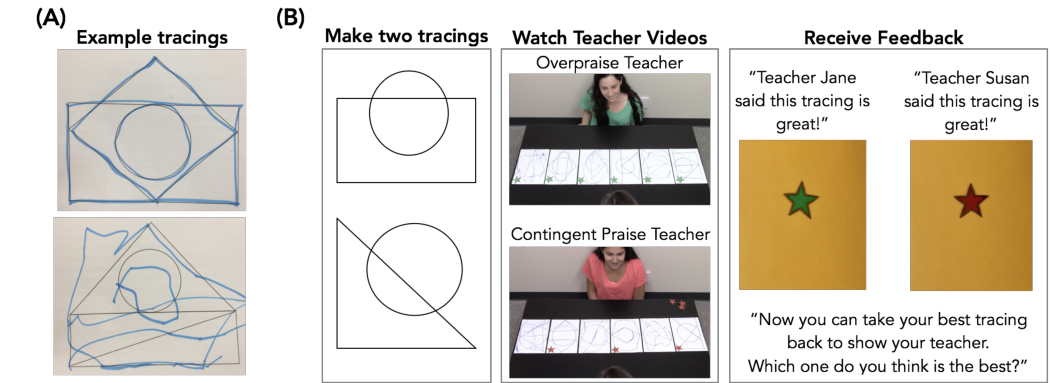
\includegraphics{figs/image-1} 

}

\caption[(A) Examples of good and bad tracings that subjects saw in the warm-up evaluation questions and teacher videos for Experiments 1-3]{(A) Examples of good and bad tracings that subjects saw in the warm-up evaluation questions and teacher videos for Experiments 1-3. (B) Procedures in Experiment 2. Experiment 3 Procedures were identical, except the Overpraise Teacher was replaced with the Inaccurate Praise Teacher.}\label{fig:image}
\end{figure*}
\end{CodeChunk}

After watching the videos, subjects were introduced to Kristen, another
student who was working on two tracings and wants to enter one of them
into a contest. Kristen received praise on one tracing (``Teacher Jane
said this is great'') from the Contingent Praise Teacher and praise on
another tracing (``Teacher Susan said this is great'') from the
Overpraise Teacher. Subjects were not given access to the tracings
themselves but only saw an envelope (presumably holding a tracing) with
Teacher Jane's green star and an envelope with Teacher Susan's red star.

Finally, subjects were asked the critical question: ``Now Kristen is
going to bring one of her tracings to a contest. Which tracing should
she bring?'' Then, subjects were asked which teacher wanted to be nice:
``One of the teachers wanted to be nice. Who was trying to be nice?''

\subsection{Results and Discussion}\label{results-and-discussion}

Our main question was whether subjects would use the teachers' prior
feedback to evaluate their feedback on the hidden tracings. Even though
each teacher provided identical evaluations on the tracings, subjects
overwhelmingly chose the tracing praised by the Contingent Praise
Teacher (87.21\%, \(p\) \textless{} .001, Binomial Test). Further,
subjects agreed that the Overpraise Teacher was \emph{trying} to be nice
(93.02\%, \(p\) \textless{} .001, Binomial Test), suggesting that
subjects did not have an overall preference for the Contingent Praise
Teacher.

Adults can distinguish between a teacher who always provides positive
feedback (Overpraise Teacher) versus a teacher who provides feedback
contingent on the quality of work (Contingent Praise Teacher). These
results suggest that adults are sensitive to the informativeness of
others' feedback: given observations of others' prior feedback, they can
differentially evaluate subsequent, identical feedback. Moreover, this
capacity to differentiate between teachers based on their prior
informativeness lead subjects to then judge which of two tracings were
better (without actually having seen the tracing).

\section{Experiment 2}\label{experiment-2}

In Experiment 2, children themselves completed two tracings, and then
watched the same videos as in Experiment 1. Children were then told that
one of their own tracings had been praised by the Contingent Praise
Teacher, and one had been praised by the Overpraise Teacher. Children
were asked to decide which of their tracings was better based on the
feedback from the teachers. We predicted that if children were sensitive
to the informativeness of praise based on each teacher's history,
children should weight the Contingent Praise Teacher's praise more
heavily, and select the tracing praised by her. On the other hand, if
children prefer to accept information from agents they perceive as
positive or friendly, they might prefer the Overpraise Teacher. Finally,
if children are not sensitive to the relative informativness of praise,
they might choose a tracing at random.

This experiment was preregistered in October 2017; the form can be found
here: \url{https://aspredicted.org/4r9dh.pdf}.

\subsection{Methods}\label{methods-1}

\subsubsection{Participants}\label{participants-1}

38 four- and five-year-olds (17 female, \(M_{Age}\)(SD) = 4.91(0.42),
Range = 4.1 - 5.91) were recruited from a local preschool. An additional
5 subjects were tested but excluded due to failure on one or two memory
check questions or a warm-up question (see Procedures below).

\subsubsection{Stimuli}\label{stimuli-1}

Children traced two templates (each had a circle and either an
overlapping triangle or square) on an 8.5 x 11'' sheet of paper with a
thick blue marker. The tracings that children evaluated during the
warm-up phase were presented on laminated sheets of paper. Children were
presented with the same videos as in Experiment 1 on a 13" Macbook Pro
laptop. Pictures of the teachers (Susan and Jane) and the student
(Johnny) were 3" x 5" respectively.

\subsubsection{Procedure}\label{procedure-1}

Children were tested in a private room inside of the preschool. The
experimenter first told children that the goal of tracing was to stay as
close to the lines as possible and demonstrated tracing a rectangle for
the child. Then, the child traced two line drawings, and the
experimenter put each tracing away into a manila envelope so the child
could not see the tracing for the remainder of the session.

Next, children were asked to evaluate two pairs of tracings to verify
that they could tell the difference between good and bad tracings. In
each pair, one tracing was obviously very good and the other tracing was
obviously very bad. Children were asked to judge which tracing was
better; only children who chose the better tracing in each pair were
included in analyses.

Children were then shown a picture of a student, Johnny. The
experimenter told children that Johnny was working on his tracings
earlier and wanted help figuring out which of his tracings were good
because he wanted to show them to his class later. Children then watched
the videos of Johnny receiving praise from the Overpraise Teacher and
the Contingent Praise Teacher (the same videos used in Experiment 1; the
teachers were referred to as Teacher Jane and Teacher Susan). After
watching each video, to verify that children understood and remembered
each teacher's pattern of praise, children were shown a still frame of
the video (with no stars on the drawings) and were asked which tracings
the teacher said were great. Children responded by pointing to the
tracings. If children incorrectly pointed to a tracing or missed a
tracing, then the video was replayed and the memory check question was
asked again. Only children who passed the memory check question by the
second attempt were included in analyses.

After children watched the videos of the teachers and responded to the
memory checks, the experimenter told the child that Teacher Jane and
Teacher Susan were close by and they could give feedback on the
subject's tracings from earlier. The experimenter left the room for 15
seconds with the envelopes containing the child's tracings and then
returned. The experimenter said ``Teacher Jane looked at this tracing
and said that this one is great'' and ``Teacher Susan looked at this
tracing and said that this one is great'' (each envelope had the
teacher's sticker on it). Finally, with the tracings still in the
envelopes, the experimenter asked the child the critical question: ``Now
you can bring back your best tracing to show your teacher! Which one do
you think is the best?'' Children responded by pointing to one of the
envelopes.

\begin{CodeChunk}
\begin{figure*}[h]

{\centering 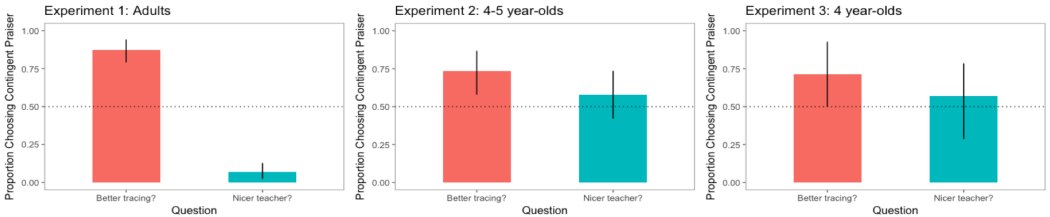
\includegraphics{figs/results_adult-1} 

}

\caption[Results of Experiment 1, 2, and 3]{Results of Experiment 1, 2, and 3.}\label{fig:results_adult}
\end{figure*}
\end{CodeChunk}

\subsection{Results and Discussion}\label{results-and-discussion-1}

Only children who passed the initial evaluation questions and the memory
check questions for each teacher video after the first or second attempt
were included in the following analyses. Our main question was which
tracing children thought was better: the tracing praised by the
Overpraise Teacher or the tracing praised by the Contingent Teacher.
Since children could not see which of their tracings was in each
envelope, the teachers' praise was the only criteria available to
children to evaluate which of their tracings was better.

We found that children were significantly more likely to choose the
drawing that had been praised by the Contingent Praise Teacher (73.68\%,
\(p\) = 0.005). Children's age did not predict their preference for the
Contingent Praise Teacher (\(B\) = 0.009, \(z\) = 0.915, \(p\) = 0.992).

Thus, even preschool-aged children appear to be sensitive to the
informativity of praise based on whether the agent has a history of
contingent praise or not. Importantly, this means that the majority of
children were able to override any positivity bias and avoid selecting
the drawing associated with the Overpraise teacher, who might have been
perceived as more nice or likeable.

Notably, in this experiment, teachers patterns' of praise differed in
two important ways. First, they differed in their contingency on
\emph{quality} --- the Contingent Teacher only praised tracings that
were objectively better, while the Overpraise teacher praised all
tracings independent of quality. Secondly, they differed in the
\emph{quantity} of tracings praised --- the Contingent teacher praised
only three out of the six tracings present, while the Overpraise teacher
praised all six. Are children sensitive to the informativity of praise
when the total amount of praise is held constant, but the accuracy of
the feedback differs? We addressed this question in Experiment 3.

\section{Experiment 3}\label{experiment-3}

\subsection{Methods}\label{methods-2}

\subsubsection{Participants}\label{participants-2}

12 4-5 year-olds (10 female, \(M_{Age}\)(SD) = 4.68(0.23), Range = 4.34
- 4.96) were recruited from a local preschool. An additional XX subjects
were tested but excluded due to failure on one or two memory check
questions or a warm-up question.

\subsubsection{Stimuli and Design}\label{stimuli-and-design}

Stimuli were identical to Experiment 2 except the Overpraise Teacher's
video was replaced with the Inaccurate Praise Teacher's video. In the
Inaccurate Praise video, the layout and order of tracing were the same
as in the Contingent and Overpraise Teacher's video, but the teacher
praised and gave stars to the worse tracings and provided a neutral
response to the better tracings.

\subsubsection{Procedure}\label{procedure-2}

The procedure was identical to Experiment 2. As in Experiment 2, the
order of the Teacher videos and actor playing each type of teacher was
counterbalanced.

\subsection{Results and Discussion}\label{results-and-discussion-2}

Our main question was whether children are sensitive to the contingency
of praise on products of better quality, controlling for the frequency
of praise.

\ldots{}

\section{General Discussion}\label{general-discussion}

In three experiments, we examined how children and adults evaluate the
informativeness of others' praise and use it to determine the quality of
their own or others' work. Experiment 1 confirms that adults
differentiate between a teacher who \textit{always} provides praise
irrespective of the quality of the product and a teacher who provides
praise contingent on the quality. Experiment 2 shows that 4-5 year-old
children distinguish between these patterns of praise and weigh the
Contingent Teacher's feedback more heavily in deciding which of their
two tracings is better. Experiment 3 shows that when the amount of
praise and contents of evaluation are held constant, 4 year-olds prefer
evaluations from teachers who provide more accurate evaluations. These
findings suggest that young children spontaneously evaluate the
informativeness of others' praise based on the contingency between
praise and quality, and that when assessing their own work, children
give more weight to praise from informative teachers.

Children's preference for the Contingent Praise Teacher is relatively
weak compared with adults' preference. There are a few possible
explanations for this discrepancy: (1) young children have relatively
minimal experience evaluating products they have created, (2) they also
have minimal experience in receiving neutral or negative feedback so
they might have difficulty reasoning about its informational value, and
(3) they might have a more difficult time inhibiting a desire to
interact or agree with positively valenced agents. Since children gain
more experience with receiving performance feedback and evaluating their
own work in elementary school, older children may show a stronger
preference for learning from teachers who provide accurate, contingent
praise.

In this study, we intentionally provided a \textit{contrast} between two
teachers who vary in their informativeness and accuracy. However, when
learning novel words, preschool-aged children have been observed to
trust even inaccurate, unreliable informants in the absence of an
accurate or informative adult (Jaswal, Croft, Setia, \& Cole, 2010,
Vanderbilt, Heyman, \& Liu (2014)). Recent work has suggested that young
children need access to relevant alternatives to compute pragmatic
implicatures (Barner, Brooks, \& Bale, 2011, Skordos \& Papafragou
(2016)) or evaluate the informativeness of pedagogical demonstrations
(Gweon \& Asaba, 2017). Thus, without the alternative of an accurate,
contingent praiser, young children might be willing to trust a teacher
who provides inaccurate or overpraise. It might be important for young
children to witness multiple informants to most effectively evaluate
them (by better understanding what the teachers \textit{could} have
said); future work should explore these possibilities.

Further, children were asked to evaluate two tracings endorsed by each
teacher. One open question is whether young children might
differentially weight praise based on their own goals in relation to the
task. Here, the learner's goal in the video demonstration (``Johnny
wants help figuring out which tracings are good because he wants to show
them to his class later'') and the subject's goal (``Now you can bring
back your best tracing to show your teacher'') was made explicit by the
experimenter. However, learners may have diverse goals in approaching
adults or teachers for help -- they could want honest evaluations of the
quality of their work and suggestions on how to improve, or they might
seek affirmation of their efforts and attempts without any evaluations
on the work, and so on.

These goals could depend on children's sense of their competence in a
task or domain; children who are just learning a new task might want
more affirmation and positivity while children who are fine-tuning their
abilities might want more constructive feedback. Children's need for
accurate feedback might also depend on their interpretation of the
activity; if they perceive the activity to be just for fun, it may not
be important to get accurate feedback, but if they believe the objective
quality of their work matters, for example, because it will be entered
in a contest or receive a grade, they might place more weight on
informative feedback. Future research that manipulates children's
task-related goals will be needed to address these possibilities.

When evaluating their tracings in this task, children did not have
visual access to each tracing, so they could only use the teacher's
evaluation and prior observations of the teacher to make the judgment.
How do children integrate their own beliefs about the quality of a piece
of work with a teacher's evaluation? One possibility is that children
might put more weight on their own beliefs when they are more certain
about how well they are doing; this certainty could rely jointly on task
characteristics (e.g., the product having an objective measure for
quality such that the ``true'' state is more obvious) and the child's
metacognitive awareness of their own skill or performance in the given
domain. Furthermore, we plan to investigate how others' feedback might
differentially influence not only product evaluations but also
subsequent learning efforts and persistence on various tasks. Recent
work has shown that infants' and young children's observations of
others' attempts influences their effort and persistence (Leonard, Lee,
\& Schulz, 2017, Magid \& Schulz (2015)).

Overall, the present work demonstrates that young children monitor the
contingency of others' praise with the quality of the work they are
evaluating, and use this information to interpret the informational
value of subsequent praise. This is likely a critical skill, as both
children and adults constantly receive praise that might be motivated by
different goals and levels of competence. Accurately representing the
informational value of this praise should allow children to gain
insights into their personal strengths and weaknesses and guide their
learning accordingly.

\section{Acknowledgements}\label{acknowledgements}

We thank Molly Irvin for her assistance with data collection, and Athena
Braun, Fernanda Kramer, and Johnny Matheou for their help in stimuli
creation. We also thank the parents and families of Bing Nursery School
for their support. This work was supported by an NSFGRFP to MA, {[}{]}
to EH, and Stanford Psych-Summer funding to HQ and BA.

\section{References}\label{references}

\setlength{\parindent}{-0.1in} \setlength{\leftskip}{0.125in} \noindent

\hypertarget{refs}{}
\hypertarget{ref-barner2011accessing}{}
Barner, D., Brooks, N., \& Bale, A. (2011). Accessing the unsaid: The
role of scalar alternatives in children's pragmatic inference.
\emph{Cognition}, \emph{118}(1), 84--93.

\hypertarget{ref-bascandziev2014beauty}{}
Bascandziev, I., \& Harris, P. L. (2014). In beauty we trust: Children
prefer information from more attractive informants. \emph{British
Journal of Developmental Psychology}, \emph{32}(1), 94--99.

\hypertarget{ref-birch2008three}{}
Birch, S. A., Vauthier, S. A., \& Bloom, P. (2008). Three-and
four-year-olds spontaneously use others' past performance to guide their
learning. \emph{Cognition}, \emph{107}(3), 1018--1034.

\hypertarget{ref-boseovski2012trust}{}
Boseovski, J. J. (2012). Trust in testimony about strangers: Young
children prefer reliable informants who make positive attributions.
\emph{Journal of Experimental Child Psychology}, \emph{111}(3),
543--551.

\hypertarget{ref-boseovski2017role}{}
Boseovski, J. J., Marble, K. E., \& Hughes, C. (2017). Role of
expertise, consensus, and informational valence in children's
performance judgments. \emph{Social Development}, \emph{26}(3),
445--465.

\hypertarget{ref-brummelman2014s}{}
Brummelman, E., Thomaes, S., Orobio de Castro, B., Overbeek, G., \&
Bushman, B. J. (2014). ``That's not just beautiful---That's incredibly
beautiful!'' the adverse impact of inflated praise on children with low
self-esteem. \emph{Psychological Science}, \emph{25}(3), 728--735.

\hypertarget{ref-gweon2017order}{}
Gweon, H., \& Asaba, M. (2017). Order matters: Children's evaluation of
underinformative teachers depends on context. \emph{Child Development}.

\hypertarget{ref-gweon2014children}{}
Gweon, H., Shafto, P., \& Schulz, L. (2014). Children consider prior
knowledge and the cost of information both in learning from and teaching
others. In \emph{Proceedings of the cognitive science society} (Vol.
36).

\hypertarget{ref-hamlin2007social}{}
Hamlin, J. K., Wynn, K., \& Bloom, P. (2007). Social evaluation by
preverbal infants. \emph{Nature}, \emph{450}(7169), 557--559.

\hypertarget{ref-harris2011young}{}
Harris, P. L., \& Corriveau, K. H. (2011). Young children's selective
trust in informants. \emph{Philosophical Transactions of the Royal
Society of London B: Biological Sciences}, \emph{366}(1567), 1179--1187.

\hypertarget{ref-hembacher2014don}{}
Hembacher, E., \& Ghetti, S. (2014). Don't look at my answer: Subjective
uncertainty underlies preschoolers' exclusion of their least accurate
memories. \emph{Psychological Science}, \emph{25}(9), 1768--1776.

\hypertarget{ref-henderlong2002effects}{}
Henderlong, J., \& Lepper, M. R. (2002). The effects of praise on
children's intrinsic motivation: A review and synthesis.
\emph{Psychological Bulletin}, \emph{128}(5), 774.

\hypertarget{ref-jaswal2010young}{}
Jaswal, V. K., Croft, A. C., Setia, A. R., \& Cole, C. A. (2010). Young
children have a specific, highly robust bias to trust testimony.
\emph{Psychological Science}, \emph{21}(10), 1541--1547.

\hypertarget{ref-johnston2015children}{}
Johnston, A. M., Mills, C. M., \& Landrum, A. R. (2015). How do children
weigh competence and benevolence when deciding whom to trust?
\emph{Cognition}, \emph{144}, 76--90.

\hypertarget{ref-kanouse1981semantics}{}
Kanouse, D. E., Gumpert, P., \& Canavan-Gumpert, D. (1981). The
semantics of praise. \emph{New Directions in Attribution Research},
\emph{3}, 97--115.

\hypertarget{ref-koenig2004trust}{}
Koenig, M. A., Clément, F., \& Harris, P. L. (2004). Trust in testimony:
Children's use of true and false statements. \emph{Psychological
Science}, \emph{15}(10), 694--698.

\hypertarget{ref-lane2013informants}{}
Lane, J. D., Wellman, H. M., \& Gelman, S. A. (2013). Informants' traits
weigh heavily in young children's trust in testimony and in their
epistemic inferences. \emph{Child Development}, \emph{84}(4),
1253--1268.

\hypertarget{ref-leonard2017infants}{}
Leonard, J. A., Lee, Y., \& Schulz, L. E. (2017). Infants make more
attempts to achieve a goal when they see adults persist. \emph{Science},
\emph{357}(6357), 1290--1294.

\hypertarget{ref-magid2015quit}{}
Magid, R., \& Schulz, L. (2015). Quit while you're ahead: Preschoolers'
persistence and willingness to accept challenges are affected by social
comparison. In \emph{CogSci}.

\hypertarget{ref-mueller1998praise}{}
Mueller, C. M., \& Dweck, C. S. (1998). Praise for intelligence can
undermine children's motivation and performance. \emph{Journal of
Personality and Social Psychology}, \emph{75}(1), 33.

\hypertarget{ref-ronfard2017preschoolers}{}
Ronfard, S., \& Lane, J. D. (2017). Preschoolers continually adjust
their epistemic trust based on an informant's ongoing accuracy.
\emph{Child Development}.

\hypertarget{ref-schneider1998performance}{}
Schneider, W. (1998). Performance prediction in young children: Effects
of skill, metacognition and wishful thinking. \emph{Developmental
Science}, \emph{1}(2), 291--297.

\hypertarget{ref-skordos2016children}{}
Skordos, D., \& Papafragou, A. (2016). Children's derivation of scalar
implicatures: Alternatives and relevance. \emph{Cognition}, \emph{153},
6--18.

\hypertarget{ref-vanderbilt2014absence}{}
Vanderbilt, K. E., Heyman, G. D., \& Liu, D. (2014). In the absence of
conflicting testimony young children trust inaccurate informants.
\emph{Developmental Science}, \emph{17}(3), 443--451.

\hypertarget{ref-yoon2016talking}{}
Yoon, E. J., Tessler, M. H., Goodman, N. D., \& Frank, M. C. (2016).
Talking with tact: Polite language as a balance between kindness and
informativity. In \emph{Proceedings of the 38th annual conference of the
cognitive science society}. Cognitive Science Society.

\end{document}
